% ------------------------------------------------------------------------
% 70. Discussion
% ------------------------------------------------------------------------

\chapter{Discussion}
\label{chap:discussion}

Designing, deploying and implementing a robust and scalable unmanned aerial system running on the cloud can be a challenging task given how many components involved that have to talk to each other in the system. Making sure that all components talk has been one of the main challenges during the project implementation.

The cloud component part has specifically posed quite a challenge to make sure that all the components can talk, ensuring that proper firewall and traffic rules are set was not easy at first, until the whole VPC traffic log started being captured and analysed. VPC flow log, an AWS network logging feature that logs all traffic flowing through all network interfaces throughout the VPC, was used to analyse the traffic. The logs would expose how traffic would flow and would indicate where traffic was being blocked. This helped then with the design of the firewall rules.

\begin{figure}[H]
    \centering 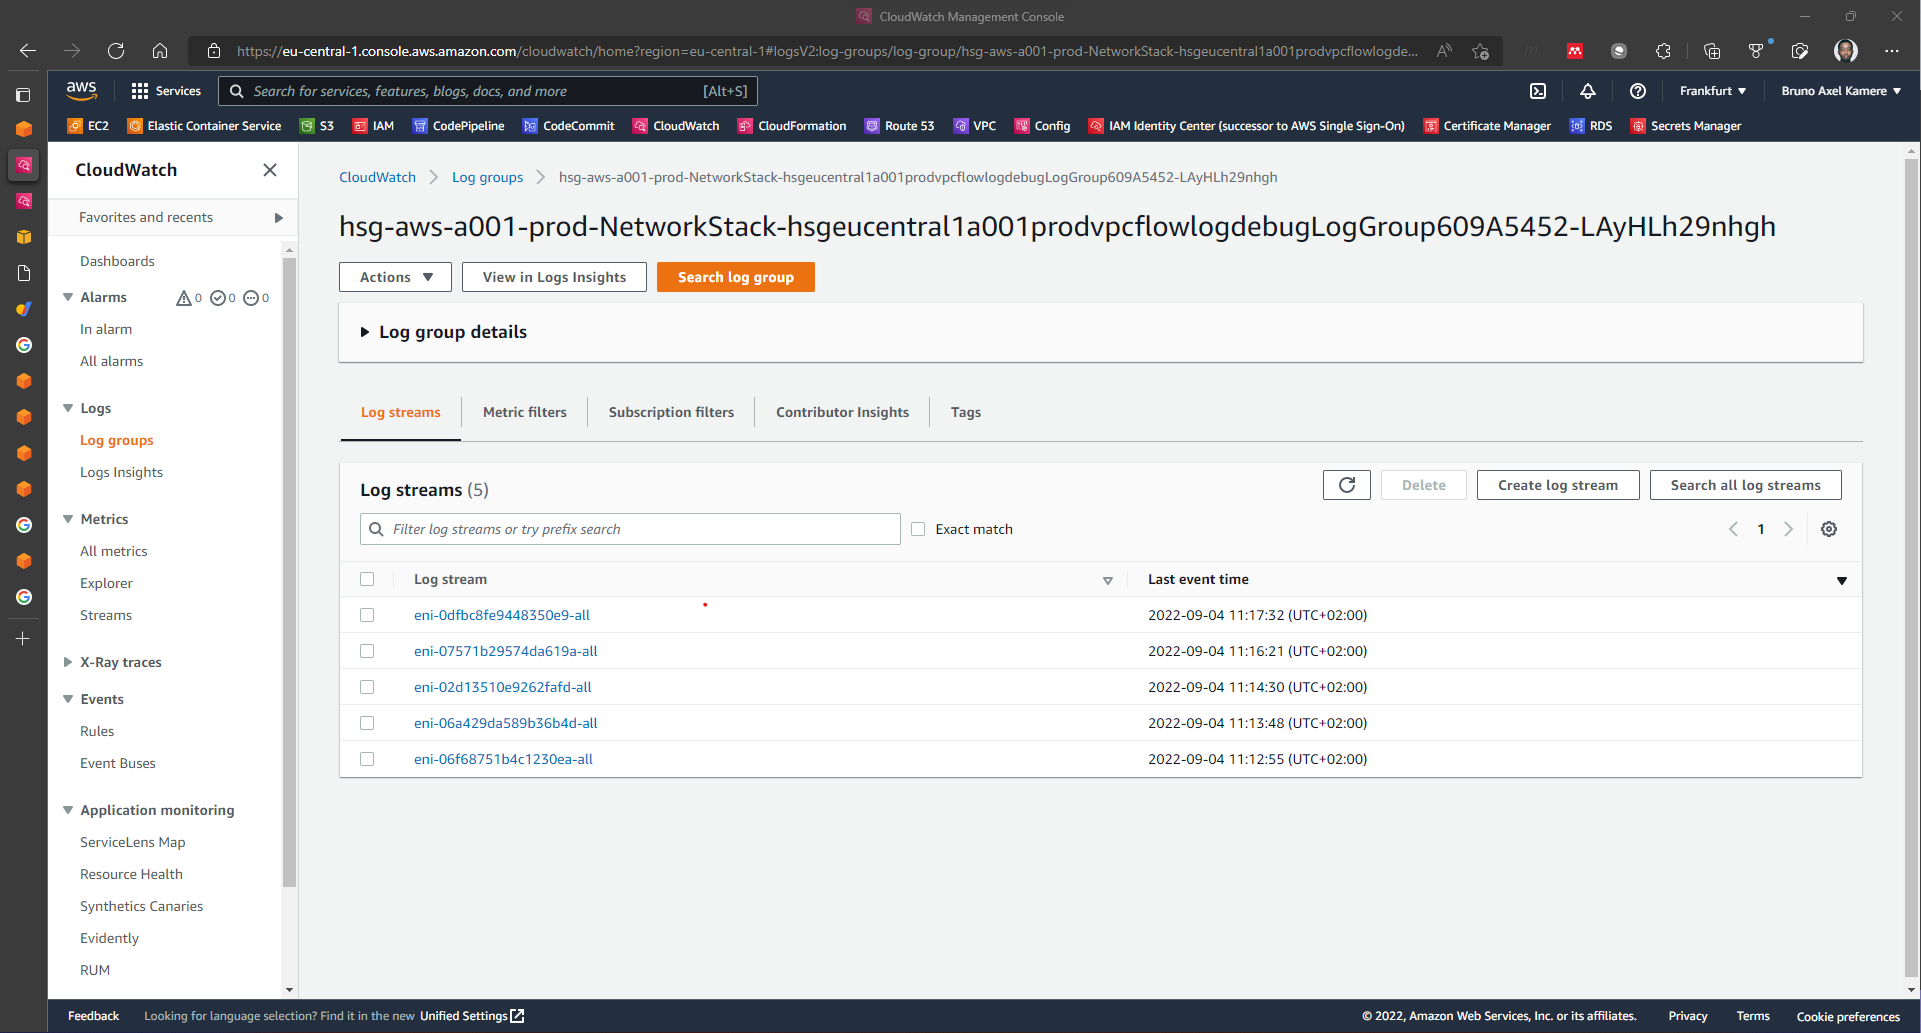
\includegraphics[width=1\linewidth]{cloud_watch_vpc_flow_log_log_groups.png}
    \caption{AWS CloudWatch VPC flow log - log groups. [Own work.]}
    \label{fig:cloud-watch-vpc-flow-log-log-groups}
    % Removed as requested by Tomasz
    % \source{Own work.}
\end{figure}

\begin{figure}[H]
    \centering 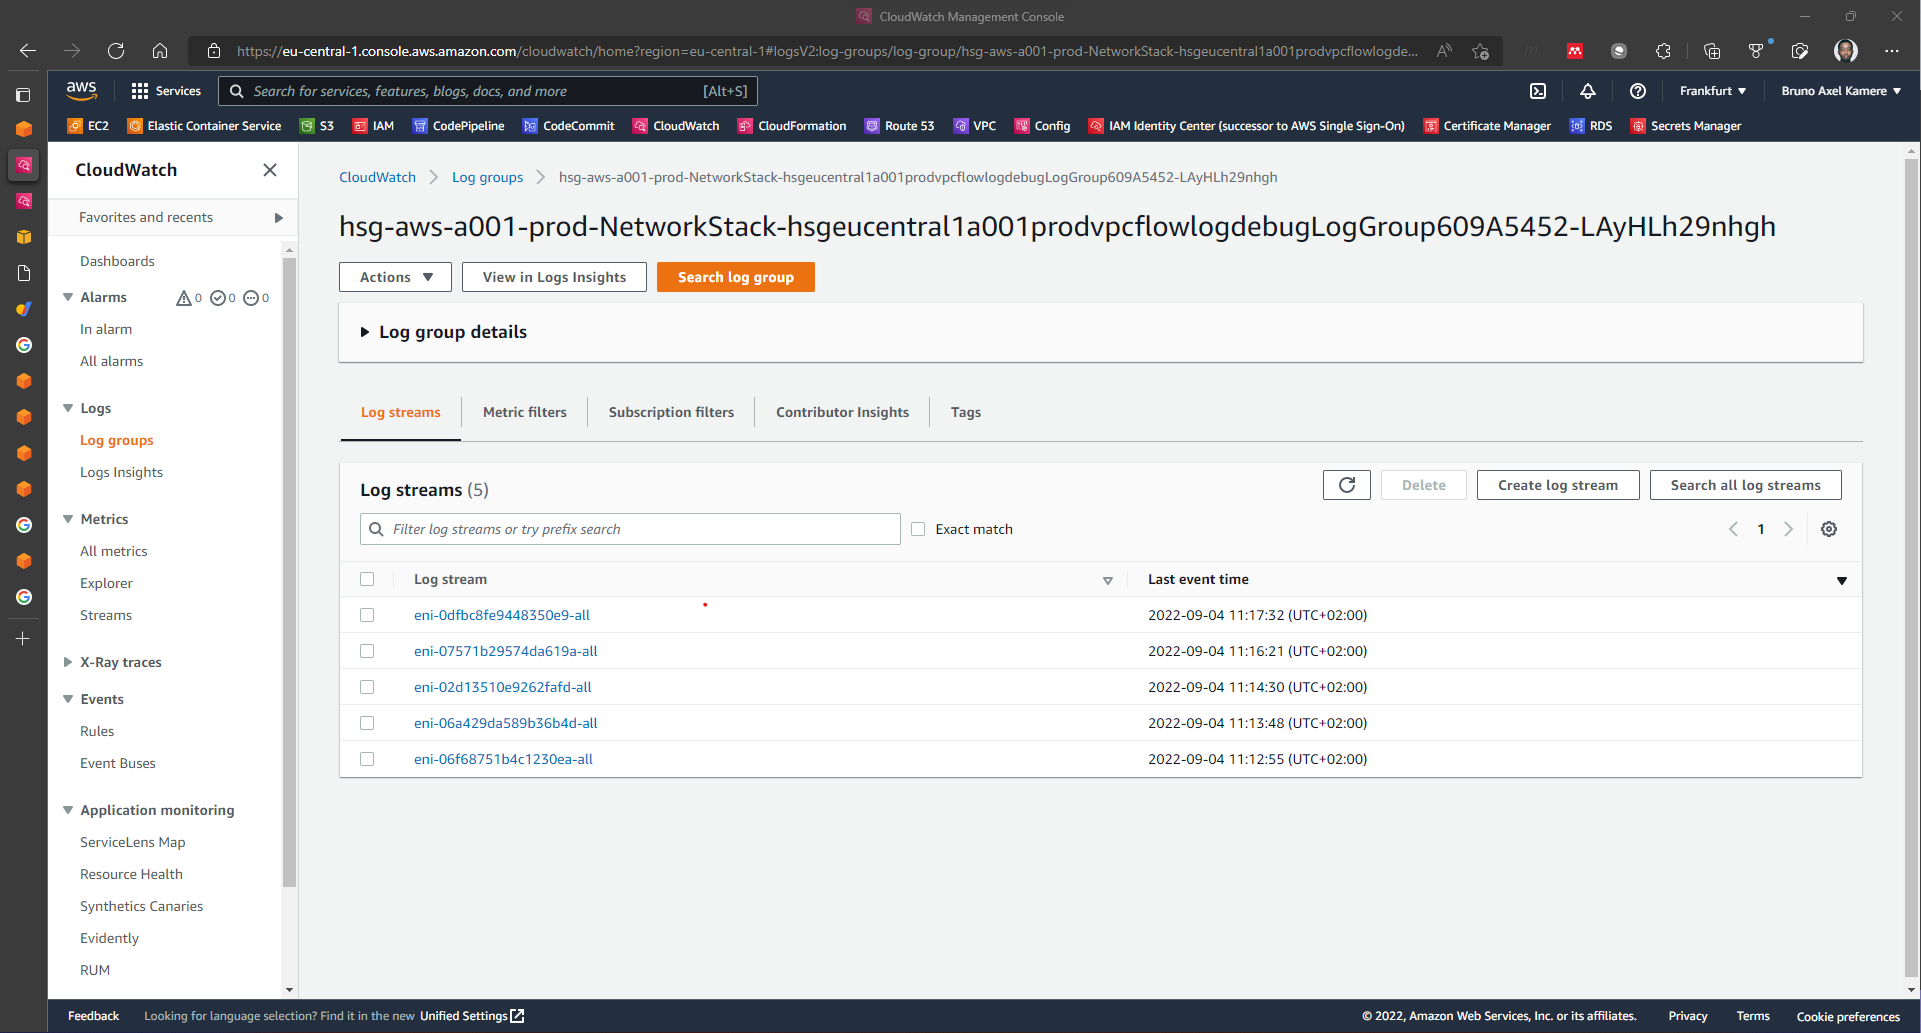
\includegraphics[width=1\linewidth]{cloud_watch_vpc_flow_log_log_events.png}
    \caption{AWS CloudWatch VPC flow log - log events. [Own work.]}
    \label{fig:cloud-watch-vpc-flow-log-log-events}
    % Removed as requested by Tomasz
    % \source{Own work.}
\end{figure}

\begin{figure}[H]
    \centering 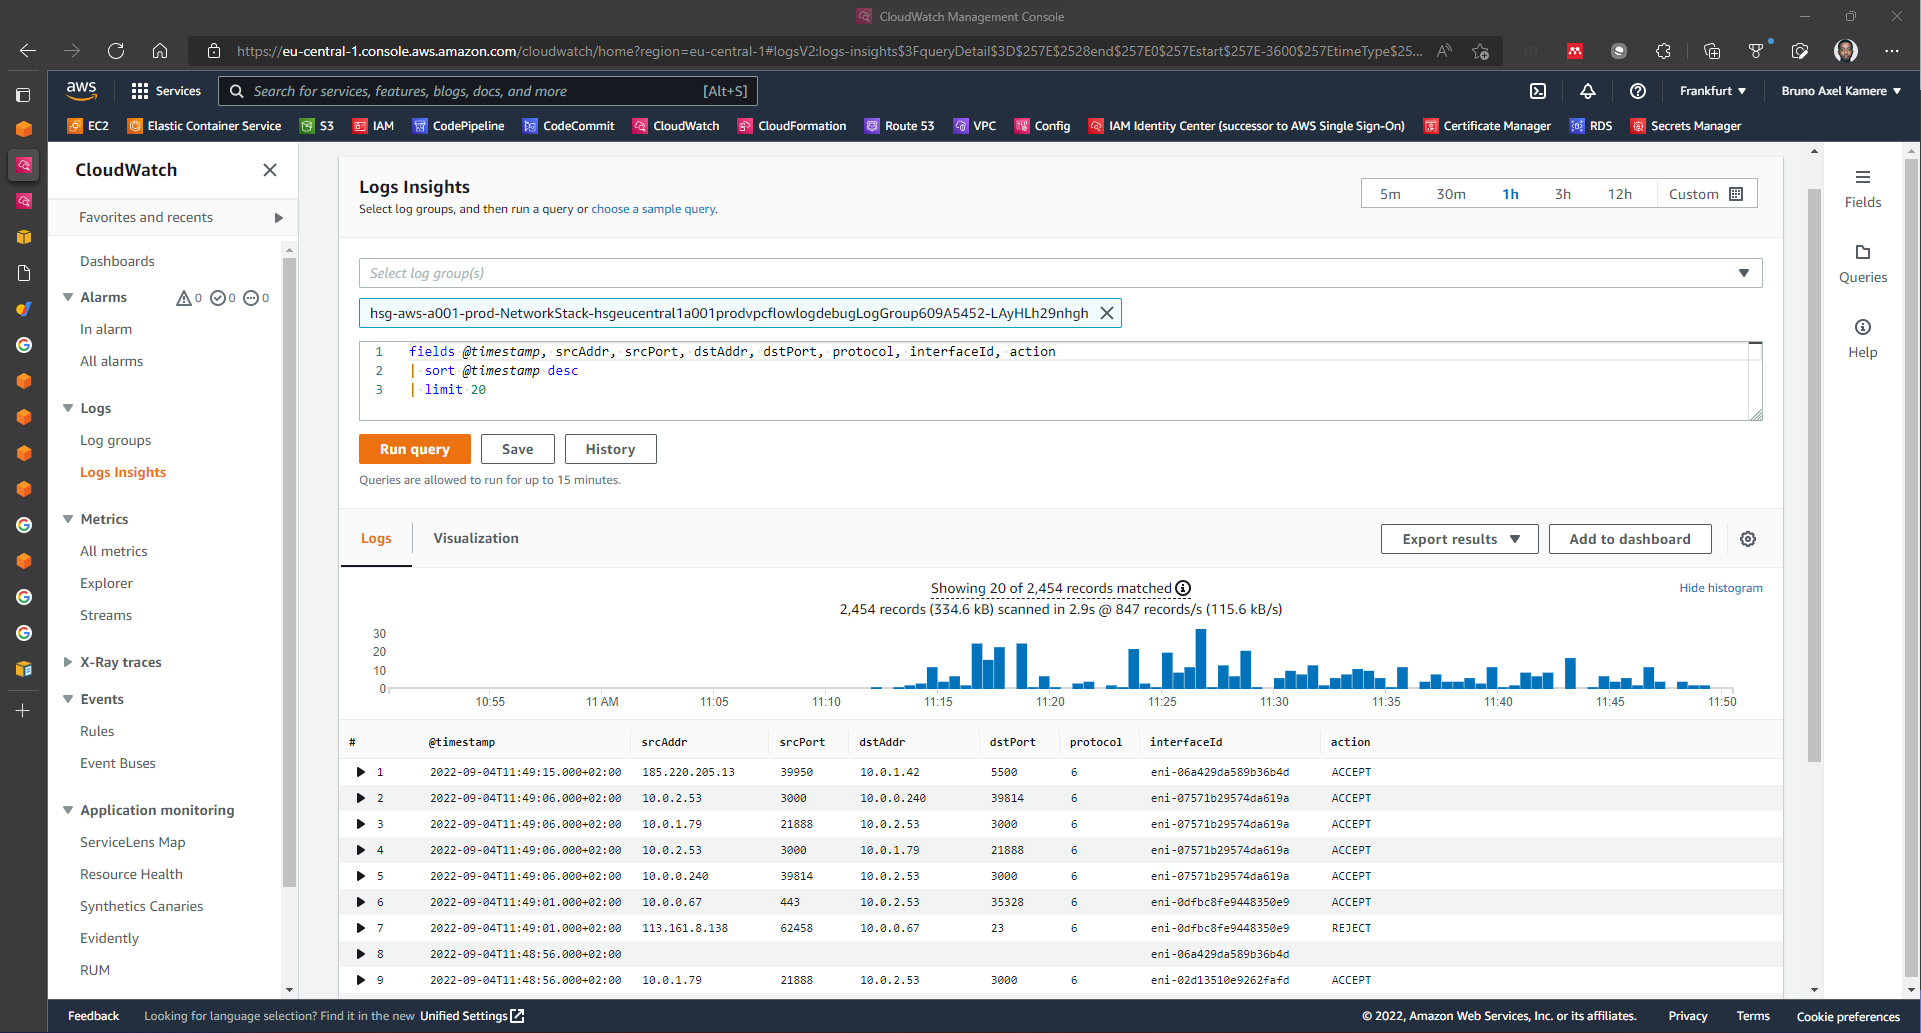
\includegraphics[width=1\linewidth]{cloud_watch_vpc_flow_log_logs_insights.png}
    \caption{AWS CloudWatch VPC flow log - log insights. [Own work.]}
    \label{fig:cloud-watch-vpc-flow-log-log-insights}
    % Removed as requested by Tomasz
    % \source{Own work.}
\end{figure}

Other than the networking aspect on AWS, integrating the UAV itself  was also quite challenging. As mentioned throughout this document, the initial idea was to build the solution with physical UAV parts. They were even available, but some parts were missing and due to how difficult it was to find them on the market, in a sense that they had to be ordered from places like China and would take some time to be delivered, it became a blocker to progress the project with actual UAV hardware. The UAV was then simulated, as described in section \ref{sec:simulation}. Simulating the UAV was not that much of a big challenge due to the very good documentation available.

Despite all the challenges faced, the use of the cloud in the unmanned aerial mobility sector seemed to be an area that can revolutionize and significantly contribute in the development of the sector. The use of various deployment techniques like infrastructure as code as described in section \ref{subsec:aws-cdk-setup} can also help in speeding up infrastructure deployment times, making the infrastructure agile and facilitating maintenance.

Making UAVs systems easy to deploy increases their accessibility to civilians thus improving several use case processes like agriculture irrigation, disaster management, \textit{et cetera}. Even though, making UAVs accessible to the public would bring positive outcomes, it would also bring a couple disadvantages mostly related to security and privacy. And this can be solved by setting strict policies and measures around the use of the UAVs.